\documentclass[a4paper,12pt]{classes/uuthesis}
\usepackage{times}
\usepackage[left=3cm,right=3cm,top=3cm]{geometry}
\usepackage{algpseudocode}
\usepackage{algorithm}
\usepackage{graphicx}
\usepackage{multirow}
\usepackage{amsmath}
\usepackage{amssymb}
\usepackage{float}
\usepackage{hyperref}
\usepackage{caption}
\usepackage{multicol}
%\setcounter{secnumdepth}{2}
\usepackage{tcolorbox}
\usepackage{setspace}
\usepackage{lipsum}
\usepackage{titlesec}
\usepackage{parskip}
\usepackage{ragged2e}
\usepackage{hyperref}
\usepackage{breakurl} % or use \url{}
\usepackage{tikz}
\usetikzlibrary{arrows.meta,positioning}

% ============================================
% CHAPTER TITLE STYLE (Clean Roman Chapter Numbers)
% ============================================
\usepackage{titlesec}
\titleformat{\chapter}[display]
  {\normalfont\huge\bfseries\centering}
  {Chapter \arabic{chapter}:}{1em}{}

% ============================================
% TOC Formatting
% ============================================
\usepackage{tocloft}
\renewcommand{\cftchappresnum}{CHAPTER~\Roman{chapter}:~}
\renewcommand{\cftchapaftersnum}{}
\setlength{\cftchapnumwidth}{7em} % Adjust space so titles don't overlap

% ============================================
% Numbering for sections and subsections
% ============================================
\renewcommand{\thesection}{\arabic{chapter}.\arabic{section}}
\renewcommand{\thesubsection}{\arabic{chapter}.\arabic{section}.\arabic{subsection}}
\numberwithin{figure}{chapter}
\numberwithin{table}{chapter}

% ============================================
% Project metadata (edit here; used across the front matter)
% ============================================
% Project metadata. Every front-matter page reads from these macros,
% so names, IDs, title and dates only need to be set once, here.
% Items in [BRACKETS] are placeholders still to be filled in.

% Working title (confirm with the supervisor before submission).
% Keep it to three lines in capitals: a fourth line pushes the date on the
% second title page onto a page of its own.
\newcommand{\ThesisTitle}{Volatility-Aware Deep Anomaly Detection for the Dhaka Stock Exchange: Transfer from Global Markets}
\newcommand{\ThesisTitleUpper}{VOLATILITY-AWARE DEEP ANOMALY DETECTION FOR THE DHAKA STOCK EXCHANGE: TRANSFER FROM GLOBAL MARKETS}

% Students
\newcommand{\StudentOneName}{MD. HASIBUL HASAN}
\newcommand{\StudentOneID}{2233081164}
\newcommand{\StudentOneEmail}{hasibul.h@uttarauniversity.edu.bd}
\newcommand{\StudentTwoName}{MOST. TASLIMA AKTER TONNE}
\newcommand{\StudentTwoID}{2233081197}
\newcommand{\StudentTwoEmail}{taslima.at@uttarauniversity.edu.bd}
\newcommand{\StudentThreeName}{ARAFAT HOSSAIN}
\newcommand{\StudentThreeID}{2233081189}
\newcommand{\StudentThreeEmail}{arafat.h@uttarauniversity.edu.bd}

% Supervisor and committee (clearance page)
\newcommand{\SupervisorName}{Dr. Md. Shafiul Alam Chowdhury}
\newcommand{\SupervisorDesignation}{Associate Professor}
\newcommand{\CoordinatorName}{[COORDINATOR NAME]}
\newcommand{\CoordinatorDesignation}{[COORDINATOR DESIGNATION]}
\newcommand{\ExaminerName}{[EXAMINER NAME]}
\newcommand{\ExaminerDesignation}{[EXAMINER DESIGNATION]}
\newcommand{\HeadName}{[HEAD OF DEPARTMENT NAME]}
\newcommand{\HeadDesignation}{[HEAD OF DEPARTMENT DESIGNATION]}

% Dates
\newcommand{\SubmissionDate}{October, 2026}  % title, second page, declaration
\newcommand{\ClearanceDate}{October, 2026}   % clearance page
\newcommand{\CopyrightYear}{2026}

% Placeholder marker for unwritten text in the chapters
\newcommand{\todo}[1]{\textit{[TODO: #1]}}


% ============================================
% Documents
% ============================================
\begin{document}
\pagenumbering{roman}

\thispagestyle{empty}
\begin{center}


\includegraphics[width=0.45\textwidth]{logo/logo.png}
\vspace{30pt}

\Large \textbf{\ThesisTitleUpper\\}
\normalsize
\vspace{50pt}

\large
\begin{tabular}{ccc}

&Submitted By&\\
&&\\
&\MakeUppercase{\StudentOneName}\\
&\MakeUppercase{\StudentTwoName}\\
&\MakeUppercase{\StudentThreeName}&\\

\end{tabular}\\

\vspace{45pt}
\large
\begin{tabular}{ccc}
&Supervisor&\\
&&\\
&\MakeUppercase{\SupervisorName}&\\
\end{tabular}\\

\vspace{60pt}
%\hspace{5cm} \makebox[6in]{\hrulefill}\\
\large

\textbf{In Partial Fulfillment} \\
\textbf{of the Requirements for the Degree of} \\
\textbf{Bachelor of Science in Computer Science and Engineering }\\
\vspace{50pt}
\textbf{\SubmissionDate}
\end{center}


\newpage

\addcontentsline{toc}{chapter}{Title page}
\begin{center}
\Large \textbf{\ThesisTitleUpper\\}
\normalsize
\vspace{100pt}

\begin{tabular}{ccc}

%\hline\noalign{\smallskip}
&Submitted By&\\
&&\\
&\StudentOneName&\\
&Student ID: \StudentOneID&\\
&E-mail: \StudentOneEmail&\\
&&\\
&\StudentTwoName&\\
&Student ID: \StudentTwoID&\\
&E-mail: \StudentTwoEmail&\\
&&\\
&\StudentThreeName&\\
&Student ID: \StudentThreeID&\\
&E-mail: \StudentThreeEmail&\\
&&\\
&&\\
&&\\
&Supervisor&\\
&&\\
&\SupervisorName&\\

%\noalign{\smallskip}\hline
\end{tabular}\\


\vspace{80pt}
\hspace{5cm} \makebox[6in]{\hrulefill}\\
\large
\textbf{Department of Computer Science and Engineering}\\
\textbf{Uttara University} \\
\textbf{Dhaka 1230, Bangladesh}\\
\vspace{50pt}
\textbf{\SubmissionDate}
\end{center}


\newpage
\addcontentsline{toc}{chapter}{Abstract}
\chapter*{\centering Abstract}
Daily stock returns alternate between calm and turbulent periods. Deep anomaly detectors
trained on raw returns therefore tend to flag whole turbulent periods rather than
individual abnormal days, and no deep, out-of-sample anomaly detection study exists for the
Dhaka Stock Exchange (DSE). This thesis proposes a volatility-aware approach. Returns are
standardized by the conditional volatility of GARCH, EGARCH or GJR models fitted on
training data only, and an LSTM autoencoder trained on the standardized returns is compared
with the same autoencoder trained on raw returns. Because the DSE has a short clean history,
detectors are trained on global market indices and transferred to the DSE, both without
retraining and after fine-tuning. Anomaly labels come from three sources fixed before any
model is trained: known market events, extreme standardized residuals and injected
anomalies. Detectors are evaluated with event-based F1 alongside point-adjusted F1 over five
random seeds, with time-based splits and a separate analysis of calm and volatile periods.
DSE data are taken from the DSEX index from 2013 and liquid stocks, with corrections for
floor-price periods and bonus-share adjustments. A preliminary run on S\&P~500 data from
1999 to 2018 supports the design: the volatility model with the best training fit failed
residual tests on the test period, while a rule based on GARCH-standardized residuals
flagged 17 days spread across the sample, against 54 days concentrated in crisis years for
a rule on raw returns.


\newpage
\addcontentsline{toc}{chapter}{Clearance Page}
\begin{center}
\large
\textbf{\ClearanceDate}\\
\textbf{Department of Computer Science and Engineering}\\
\textbf{Uttara University}\\

\end{center}

We hereby certify that \textbf{\StudentOneName}, \textbf{\StudentTwoName}, \textbf{\StudentThreeName} students of the Department of Computer Science and Engineering (CSE) at Uttara University, have successfully completed their thesis titled "\textbf{\ThesisTitle}" in partial fulfillment of the requirements for the degree of Bachelor of Science in Computer Science and Engineering (CSE) at Uttara University.\\
\vspace{45pt}\\

\begin{tabular}{lll}
\makebox[3.3in]{\hrulefill}& \hspace{2cm} & Supervisor\\
Name: \SupervisorName &  & \\
Designation: \SupervisorDesignation &  & \\
Department of Computer Science and Engineering&  & \\
Uttara University &  & \\
&&\\
&&\\
&&\\
\makebox[3.3in]{\hrulefill}& \hspace{2cm} & Coordinator\\
Name: \CoordinatorName &  & \\
Designation: \CoordinatorDesignation  &  & \\
Department of Computer Science and Engineering&  & \\
Uttara University &  & \\
&&\\
&&\\
&&\\
\makebox[3.3in]{\hrulefill}& \hspace{2cm} & Examiner\\
Name: \ExaminerName &  & \\
Designation: \ExaminerDesignation &  & \\
Department of Computer Science and Engineering&  & \\
Uttara University &  & \\
&&\\
&&\\
&&\\
\makebox[3.3in]{\hrulefill}& \hspace{2cm} & Head of the Department\\
Name: \HeadName &  & \\
Designation: \HeadDesignation &  & \\
Department of Computer Science and Engineering&  & \\
Uttara University &  & \\
\end{tabular}\\

\newpage
\addcontentsline{toc}{chapter}{Submission Page}
\begin{center}
\large
\textbf{\SubmissionDate}\\
\textbf{Department of Computer Science and Engineering}\\
\textbf{Uttara University}\\
\end{center}

We, the undersigned, hereby declare that this project entitled “\textbf{\ThesisTitle}” presents the original thesis work of \StudentOneName, \StudentTwoName{} and \StudentThreeName. Wherever the contributions of others are involved, due acknowledgment has been made through proper citations and references. This work was carried out under the supervision of \SupervisorName, in the Department of Computer Science and Engineering (CSE) at Uttara University.\\

\vspace{60pt}
\begin{tabular}{l}
\makebox[2.0in]{\hrulefill} \\
Name: \StudentOneName \\
Student ID: \StudentOneID \\
Department of CSE \\
Uttara University \\[1.5cm]

\makebox[2.0in]{\hrulefill} \\
Name: \StudentTwoName \\
Student ID: \StudentTwoID \\
Department of CSE \\
Uttara University \\[1.5cm]

\makebox[2.0in]{\hrulefill} \\
Name: \StudentThreeName \\
Student ID: \StudentThreeID \\
Department of CSE \\
Uttara University \\
\end{tabular}


\newpage
\addcontentsline{toc}{chapter}{Copyright}
\begin{center}
    \begin{tcolorbox}[colback=white, colframe=black, boxrule=1pt, width=\textwidth, arc=5pt, auto outer arc, sharp corners=south]
    \centering

    \Large\textbf{UTTARA UNIVERSITY} \\[2em]

    \large\textit{DECLARATION OF COPYRIGHT AND AFFIRMATION OF FAIR USE OF  UNPUBLISHED RESEARCH} \\[1em]

    \normalsize{\ThesisTitleUpper} \\[2em]

  \begin{justify}  We declare that the copyright holders of this dissertation are jointly owned by the students and Uttara University (UU).\\[1em] \end{justify}

    \textcopyright{} \CopyrightYear{} \textit{\StudentOneName, \StudentTwoName, \StudentThreeName} and Uttara University (UU). All rights reserved.\\[1em]

   \begin{justify} No part of this unpublished research may be reproduced, stored in a retrieval system, or transmitted, in any form or by any means, electronic, mechanical, photocopying, recording, or otherwise without prior written permission of the copyright holder except as provided below.\\[1em] \end{justify}

    \begin{enumerate}
        \item Any material contained in or derived from this unpublished research may be used by others in their writing with due acknowledgement.
        \item UU or its library will have the right to make and transmit copies (print or electronic) for institutional and academic purposes.
        \item The UU library will have the right to make, store in a retrieval system and supply copies of this unpublished research if requested by other universities and research libraries.
    \end{enumerate}

   \begin{justify} \noindent\\[1ex] By signing this form, we acknowledged that we have read and understand the UU Intellectual Property Right and Commercialization policy.\\[2em] \end{justify}

    Affirmed by \textit{\StudentOneName} \\[2em]

    \hfill \begin{tabular}{ll}
        \rule{6cm}{0.4pt} & \rule{3cm}{0.4pt} \\
        Signature (on behalf of the team) & Date
    \end{tabular}
    \end{tcolorbox}
\end{center}


\newpage
\addcontentsline{toc}{chapter}{Dedication}
\chapter*{\centering Dedication}
\todo{Dedication (one or two sentences, chosen by the team).}


\newpage
\addcontentsline{toc}{chapter}{Acknowledgment}
 \chapter*{\centering Acknowledgment}
% Written by the team. Thank the supervisor (\SupervisorName), the examiner,
% the CSE faculty, families and friends, in your own words.
\todo{Acknowledgment, in the team's own words.}


\newpage
\addcontentsline{toc}{chapter}{Table of Contents}
\tableofcontents

\newpage
\addcontentsline{toc}{chapter}{List of Tables}
\listoftables

\newpage
\addcontentsline{toc}{chapter}{List of Figures}
\listoffigures

\newpage
\addcontentsline{toc}{chapter}{Symbols}
\chapter*{\centering Symbols}
\noindent
\begin{tabular}{p{3.0cm}p{10.0cm}}

$P_t$			&closing price (or index level) on trading day $t$;\\
$r_t$			&daily log return, $r_t = \ln(P_t / P_{t-1})$;\\
$\mu$			&conditional mean of the return;\\
$\varepsilon_t$	&return innovation, $\varepsilon_t = r_t - \mu$;\\
$\sigma_t^2$	&conditional variance of $r_t$ given information up to $t-1$;\\
$z_t$			&GARCH-standardized residual, $z_t = \varepsilon_t / \sigma_t$;\\
$\omega, \alpha, \beta$	&GARCH(1,1) constant, ARCH and GARCH coefficients;\\
$\gamma$		&leverage (asymmetry) coefficient in EGARCH and GJR models;\\
$\nu$			&degrees of freedom of the Student-$t$ innovation distribution;\\
$s_t$			&anomaly score assigned to day $t$ by a detector;\\
$\tau$			&decision threshold on the anomaly score.\\

\end{tabular}


\newpage
\addcontentsline{toc}{chapter}{Abbreviation}
\chapter*{\centering List of Abbreviation}
\noindent
\begin{tabular}{p{3.0cm}p{10.0cm}} 

AE 		& Autoencoder \\
ARCH	& Autoregressive Conditional Heteroskedasticity \\
BIC		& Bayesian Information Criterion \\
BSEC	& Bangladesh Securities and Exchange Commission \\
DSE 	& Dhaka Stock Exchange \\
DSEX	& DSE Broad Index \\
EGARCH	& Exponential GARCH \\
F1-PA	& Point-Adjusted F1 Score \\
GARCH	& Generalized Autoregressive Conditional Heteroskedasticity \\
GJR		& Glosten-Jagannathan-Runkle GARCH \\
LSTM	& Long Short-Term Memory \\
PA		& Point Adjustment \\
TSAD	& Time-Series Anomaly Detection \\

\end{tabular}


\newpage
\addcontentsline{toc}{chapter}{Appendices}
\chapter*{\centering Appendices}
\begin{tabular}{p{3.0cm}p{9.0cm}p{2.0cm}} 
APPENDIX A & Research Publications & [page]\\ %manually typed page
\\
APPENDIX B & Success \& Achievement & [page]\\ %manually typed page
\end{tabular}


\newpage
\pagenumbering{arabic}
\chapter[Introduction]{Introduction}
% Chapter 1: Introduction.

\section{Background of the Study}
Stock exchanges and regulators watch for trading days that depart from normal market
behaviour, such as sudden crashes, manipulated prices or reactions to regulatory news.
Finding such days automatically is an anomaly detection problem, and deep learning models
that learn normal behaviour from data and score departures from it are now widely used for
time series~\cite{malhotra2016lstm,hundman2018detecting,xu2018unsupervised}.

Financial returns are a difficult setting for these models. Their variance is not constant:
large moves cluster in turbulent periods and small moves in calm ones, a property captured
by ARCH and GARCH models~\cite{engle1982autoregressive,bollerslev1986generalized}. A 3\%
fall is ordinary in a crisis and exceptional in a quiet year. A detector that judges every
day on the same scale will mark crisis periods as anomalous and miss unusual days in calm
periods.

The difficulty is greater in emerging and frontier markets. The Dhaka Stock Exchange (DSE)
in Bangladesh has a broad index, DSEX, only from January 2013. Its prices are not adjusted
for the frequent bonus share issues of listed firms, and for long stretches between 2020 and
2024 the Bangladesh Securities and Exchange Commission (BSEC) imposed floor prices that froze
many stocks. Little clean data is available to train a detector on the DSE alone.

\section{Problem Statement}
Published DSE volatility studies fit GARCH-family models in
sample~\cite{siddikee2016volatility,haque2021modeling}, and published anomaly detection
studies on stock data do not adjust their inputs for volatility
clustering~\cite{golmohammadi2015time,mariani2021autoencoder}. Among the work reviewed in
Chapter~2, none applies a deep anomaly detector to the DSE, none uses GARCH-standardized
returns as a detector's input, and none transfers an anomaly detector from developed markets
to a frontier market. A further problem concerns evaluation. Many time-series anomaly
detection results are reported with point adjustment, which can make random scores look
competitive~\cite{kim2022towards}, and the size of this effect on financial data is unknown.

As a result, there is no tested method for flagging abnormal trading days on the DSE that
accounts for changing volatility, and no reliable estimate of how well such a method would
perform.

\section{Research Objectives}

\subsection*{General Objective}
To develop and evaluate a volatility-aware deep anomaly detector for daily stock returns
that can be transferred from global market indices to the Dhaka Stock Exchange.

\subsection*{Specific Objectives}
\begin{enumerate}
    \item To build a leakage-safe data pipeline for global index and DSE daily data,
    including corrections for DSE floor prices, bonus shares and price limits.
    \item To fit GARCH, EGARCH and GJR models on training data and select one on
    out-of-sample residual diagnostics.
    \item To construct anomaly labels from known events, extreme standardized residuals and
    injected anomalies, with the rules fixed before any detector is trained.
    \item To compare an LSTM autoencoder trained on raw returns with the same model trained
    on GARCH-standardized returns, against statistical and classical baselines.
    \item To measure how well detectors trained on global indices transfer to the DSE, with
    and without fine-tuning.
    \item To report event-based and point-adjusted scores over several random seeds, with an
    analysis by volatility regime.
\end{enumerate}

\section{Research Questions and Hypotheses}
\begin{enumerate}
    \item[\textbf{RQ1.}] Does standardizing returns by GARCH-family conditional volatility
    improve deep anomaly detection on stock returns?

    \textit{H1:} An autoencoder trained on GARCH-standardized returns achieves a higher
    event-based F1 and raises fewer false alarms in high-volatility periods than the same
    autoencoder trained on raw returns.

    \item[\textbf{RQ2.}] Can an anomaly detector trained on global market indices be
    transferred to the DSE?

    \textit{H2:} A detector trained on global indices and applied to DSE data without
    retraining outperforms the statistical baselines on the DSE, and fine-tuning on DSE
    training data improves it further.

    \item[\textbf{RQ3.}] How much does point adjustment inflate reported anomaly detection
    performance on financial data?

    \textit{H3:} Point-adjusted F1 is substantially higher than event-based F1 for every
    detector, including the simple baselines.
\end{enumerate}

\section{Scope and Delimitation}
The study uses daily data only, because free intraday DSE data do not exist. On the DSE it
covers the DSEX index from its launch in January 2013 and 10 to 20 liquid stocks chosen by
turnover. Periods under BSEC floor prices are treated as a separate regime. Global market
indices, starting with the S\&P~500, serve as the source domain for transfer. Market
manipulation cases, order-book data, and news or text data are outside the scope.

\section{Significance of the Study}
For the DSE, the study would provide the first out-of-sample test of deep anomaly detection
among the work reviewed, together with documented handling of the exchange's data problems.
For anomaly detection on financial data more generally, it tests whether removing the
volatility level from the input changes which days a deep detector flags, and it measures
how much point adjustment overstates performance. The code will be public, and the labelled
DSE series will be released if the data licence allows, which would give later work a
financial benchmark that current collections lack~\cite{paparrizos2022tsb,schmidl2022anomaly}.

\section{Definition of Terms}
\begin{itemize}
    \item \textbf{Anomaly:} a trading day whose return is unusual relative to the
    volatility of its own period, or that coincides with a documented market event.
    \item \textbf{Volatility clustering:} the tendency of large price changes to follow
    large changes and small changes to follow small ones.
    \item \textbf{GARCH-standardized return:} the return innovation divided by its
    conditional standard deviation, $z_t = \varepsilon_t / \sigma_t$.
    \item \textbf{Transfer learning:} training a model on one domain, here global market
    indices, and applying it, with or without further training, to another, here the DSE.
    \item \textbf{Point adjustment:} an evaluation rule that counts every point of a
    labelled anomalous segment as detected if any one of its points is detected.
\end{itemize}

\section{Organization of the Thesis}
Chapter~2 reviews related work on volatility modelling, financial and time-series anomaly
detection, evaluation practice and transfer learning. Chapter~3 describes the proposed data
pipeline, labels, models and evaluation protocol. Chapter~4 reports preliminary results and
the expected outcomes. Chapter~5 sets out the work plan, risks and fallbacks.


\chapter{Literature Review}
% Chapter 2: Literature Review (the paper plan's "Related Work").
% Source: /mnt/project-files/literature/literature_table.xlsx (Papers and Gaps tabs).
% Limitations marked "Observed" in that table are the team's reading, not the authors'
% claims. They are written below as descriptions of what each study did, and should be
% checked against the full texts before submission.

\section{Introduction}
This chapter reviews the work this thesis builds on. Section~\ref{sec:lr-theory} sets out
the volatility models and the notion of an anomaly used throughout. Section~\ref{sec:lr-themes}
reviews seven bodies of work: hybrid GARCH and deep learning models, outliers in GARCH
estimation, volatility studies of the Dhaka Stock Exchange (DSE), anomaly detection in
financial markets, deep time-series anomaly detection, the evaluation of such detectors,
and transfer learning in finance. Section~\ref{sec:lr-gaps} lists the gaps that motivate
this study.

\section{Theoretical Background}\label{sec:lr-theory}

\subsection{Volatility Clustering and GARCH-Family Models}
Daily stock returns are close to uncorrelated, but their magnitude is not: large moves
tend to follow large moves. Engle's ARCH model~\cite{engle1982autoregressive} captured this
by letting the conditional variance depend on past squared innovations, and
Bollerslev's GARCH model~\cite{bollerslev1986generalized} added a dependence on past
conditional variance, which gives a parsimonious description of persistent volatility.
Two extensions allow negative shocks to raise volatility more than positive shocks of the
same size: EGARCH~\cite{nelson1991conditional}, which models the logarithm of the variance,
and the GJR model~\cite{glosten1993relation}, which adds a term that is active only after
negative returns. Chapter~\ref{ch:method} gives the equations used in this thesis.

Dividing each return innovation by its conditional standard deviation gives a standardized
residual, $z_t = \varepsilon_t/\sigma_t$. If the volatility model is adequate, $z_t$ has no
remaining volatility clustering, so a day with a large $|z_t|$ is unusual relative to the
volatility of its own period rather than relative to the whole sample.

\subsection{Anomalies in Financial Time Series}
\todo{Define point, contextual and collective anomalies, and state which kind this thesis
targets. Golmohammadi and Zaiane~\cite{golmohammadi2015time} is a starting point for
contextual anomalies in stock prices.}

\section{Review of Key Themes}\label{sec:lr-themes}

\subsection{GARCH Models Combined with Deep Learning}
Kim and Won~\cite{kim2018forecasting} fed the outputs of GARCH, EGARCH and EWMA models
into an LSTM and forecast the realized volatility of the KOSPI~200 index, reporting lower
errors than either the econometric models or the networks alone. Koo et
al.~\cite{koo2022hybrid} combined GARCH-type inputs with a root-type transform of the
volatility distribution before an LSTM, motivated by the observation that volatility is
concentrated near zero, so a network trained on the raw distribution fits the common
region and misses the tail. They report a 21\% reduction in RMSE over earlier LSTM-GARCH
hybrids on S\&P~500 realized volatility.

Both studies use GARCH output to improve a volatility forecast on a single index. Neither
addresses anomaly detection. The second study's motivation is relevant here: if a network
trained on raw values under-fits the tail, a transform that removes the volatility level
may help a detector separate unusual days from merely turbulent ones. This thesis tests
that idea with GARCH standardization.

\subsection{Outliers in GARCH Estimation}
Charles and Darn{\'e}~\cite{charles2005outliers} showed that outliers in daily returns
bias GARCH parameter estimates and test statistics, and proposed a procedure to detect and
correct them during estimation. Their work treats outliers as a nuisance for estimation
rather than as targets. For this thesis it has two consequences. Labelling a day as
anomalous from an extreme standardized residual is an established idea, and extreme days in
the estimation window will distort the fitted model, which is one reason the volatility
models here are estimated on the training block only.

\subsection{Volatility Studies of the Dhaka Stock Exchange}
Siddikee et al.~\cite{siddikee2016volatility} fitted GARCH(1,1) and ARCH models to the DSE
General Index (DGEN) from January 2002 to July 2013 and identified an episode of abnormal
volatility between 2009 and 2012, peaking in the first half of 2011. They report that
GARCH could not be applied in some years and used ARCH instead. Haque et
al.~\cite{haque2021modeling} fitted long-memory models (FIGARCH, FIEGARCH, FIAPARCH and
HYGARCH) to the DSEX and DSES indices and examined asymmetry through news impact curves.

Both studies are in-sample descriptions of DSE volatility. Neither evaluates models out of
sample or addresses anomaly detection. The DGEN series studied by Siddikee et al.\ was
replaced by DSEX in 2013, so their sample and the DSEX series used in this thesis do not
overlap.

\subsection{Anomaly Detection in Financial Markets}
Two surveys frame the area. Ahmed et al.~\cite{ahmed2016survey} review anomaly detection
for financial fraud, with an emphasis on clustering methods, and Hilal et
al.~\cite{hilal2022financial} review supervised, unsupervised and semi-supervised fraud
detection, including deep learning, and identify the scarcity of public labelled data as a
recurring obstacle.

Work on stock markets faces the same labelling problem. Golmohammadi and
Zaiane~\cite{golmohammadi2015time} detected contextual anomalies in S\&P~500 constituents
by comparing each stock with its peer group, and evaluated on injected synthetic anomalies
because confirmed manipulation cases were not available. On the Stock Exchange of Thailand,
Leangarun et al.~\cite{leangarun2021stock} trained an autoencoder and a GAN on normal
limit-order-book behaviour and detected five of six prosecuted manipulation cases, and
Chullamonthon et al.~\cite{chullamonthon2023ensemble} stacked an LSTM classifier and an
LSTM autoencoder with an SVM and detected all six. Six cases are too few to support
statistical comparisons between methods. Mariani et al.~\cite{mariani2021autoencoder}
applied LSTM, bidirectional LSTM and convolutional autoencoders to the IBOVESPA index and
flagged days with high reconstruction error, without a defined ground truth.

None of these studies adjusts its inputs for volatility clustering, and each is confined to
a single market.

\subsection{Deep Time-Series Anomaly Detection Methods}
Most deep detectors for time series score a point by how poorly a model trained on normal
data reconstructs or predicts it. Malhotra et al.~\cite{malhotra2016lstm} used an LSTM
encoder-decoder and scored windows by reconstruction error on sensor and medical data.
Hundman et al.~\cite{hundman2018detecting} forecast spacecraft telemetry with an LSTM and set
thresholds on the forecast errors with a nonparametric dynamic method. Xu et
al.~\cite{xu2018unsupervised} trained a variational autoencoder (Donut) on sliding windows
of web-service KPIs. Xu et al.~\cite{xu2022anomaly} proposed the Anomaly Transformer, which
scores points by an association-discrepancy criterion.

These methods were developed and tested on sensor, telemetry and operations data. None was
evaluated on financial returns, whose variance changes over time. A reconstruction-error
detector trained on raw returns will tend to score every day of a high-volatility period as
anomalous, which is the behaviour this thesis aims to measure and reduce.

\subsection{Evaluation of Time-Series Anomaly Detection}
Several papers question how these detectors are evaluated. Xu et
al.~\cite{xu2018unsupervised} introduced point adjustment: if any point inside a labelled
anomalous segment is detected, every point in the segment is counted as detected. Kim et
al.~\cite{kim2022towards} showed that under point adjustment, random anomaly scores can
match published state-of-the-art results, and proposed PA\%K, which credits a segment only
if at least $K$\% of its points are detected. Tatbul et al.~\cite{tatbul2018precision}
defined range-based precision and recall with tunable terms for existence, overlap,
position and cardinality. Paparrizos et al.~\cite{paparrizos2022volume} proposed the
threshold-free VUS-ROC and VUS-PR measures, which tolerate small lags between predicted and
true anomalies.

The benchmarks themselves have also been criticised. Wu and
Keogh~\cite{wu2023current} argue that widely used benchmarks are often trivial, have
unrealistic anomaly densities and contain labelling errors, and they released the UCR
anomaly archive. TSB-UAD~\cite{paparrizos2022tsb} and the evaluation by Schmidl et
al.~\cite{schmidl2022anomaly} compare many detectors on large collections of real and
synthetic series. Schmidl et al.\ report that no single algorithm wins and that simple
methods are often competitive. Neither collection includes financial series.

This thesis therefore reports event-based F1 alongside point-adjusted F1 and PA\%K, and
includes simple statistical baselines.

\subsection{Transfer Learning in Finance}
Koshiyama et al.~\cite{koshiyama2022quantnet} trained QuantNet, which shares a
market-agnostic layer across equity markets and adds market-specific encoders and decoders,
and measured gains in trading performance (Sharpe and Calmar ratios). Nguyen and
Yoon~\cite{nguyen2019novel} pretrained an LSTM on a large pool of stocks and fine-tuned it to
predict short-term price movements of target stocks. Both target prediction or trading
rather than detection, and neither transfers into a frontier market such as Bangladesh.

\section{Critical Analysis and Research Gaps}\label{sec:lr-gaps}
The review points to seven gaps.

\begin{enumerate}
    \item Hybrid GARCH and deep learning models are used for volatility forecasting
    \cite{kim2018forecasting,koo2022hybrid}. None of the studies reviewed uses
    GARCH-standardized returns as the input to a deep anomaly detector.
    \item Anomaly detectors applied to stock data do not adjust for volatility
    clustering~\cite{golmohammadi2015time,mariani2021autoencoder}, so calm and turbulent
    periods are scored on the same scale.
    \item Published DSE studies fit GARCH-family models in
    sample~\cite{siddikee2016volatility,haque2021modeling}. None of the studies reviewed
    applies deep or out-of-sample anomaly detection to the DSE.
    \item Cross-market transfer has been studied for trading and price
    prediction~\cite{koshiyama2022quantnet,nguyen2019novel}, not for anomaly detection into a
    frontier market.
    \item Labels in financial anomaly studies are either very few real cases
    \cite{leangarun2021stock,chullamonthon2023ensemble} or synthetic
    \cite{golmohammadi2015time}, and the shortage of public labelled data is a known
    obstacle~\cite{hilal2022financial}.
    \item The inflation caused by point adjustment has been measured on industrial and
    operations benchmarks~\cite{kim2022towards,wu2023current} but not on financial data.
    \item Large anomaly detection benchmarks contain no financial
    series~\cite{paparrizos2022tsb,schmidl2022anomaly}.
\end{enumerate}

This thesis addresses the first five directly. It compares an autoencoder on raw and on
GARCH-standardized returns, analyses false alarms by volatility regime, evaluates on DSE
data with time-based splits, transfers detectors from global indices to the DSE, and builds
labels from three sources: known market events, extreme standardized residuals and injected
anomalies. It addresses the sixth by reporting point-adjusted and unadjusted scores side by
side.

\section{Summary of Literature Review}
GARCH-family models describe DSE volatility well in sample, and deep detectors work on
sensor and operations data, but the two have not been combined for anomaly detection in
stock markets, and nothing comparable exists for the DSE. Evaluation practice in the field
also overstates performance when point adjustment is used. Chapter~\ref{ch:method} describes
the data, labels, models and evaluation protocol designed around these gaps.


\chapter{Methodology} 
% Chapter 3: Methodology (the paper plan's "Data and Labeling" and "Method").
% Project rules that hold throughout: time-based splits only, volatility models
% fitted on the training block only, fixed seeds (config.yaml, seed 42).
\label{ch:method}

\section{Introduction}
This chapter describes the data, the volatility models, the anomaly labels, the detectors
and the evaluation protocol. The study is quantitative and experimental. Two comparisons
drive it: a detector trained on raw returns against the same detector trained on
GARCH-standardized returns, and a detector trained on global market indices and applied to
the Dhaka Stock Exchange (DSE) against one trained on DSE data. Sections marked as planned
describe work that has not yet been run.

\section{Research Design}
\todo{Map each research question in Chapter 1 to the experiment that answers it.}

\section{Data Collection}

\subsection{Global Market Data}
Global index data come from Yahoo Finance through the \texttt{yfinance} Python package. The
first index used is the S\&P~500 (\texttt{\^{}GSPC}), daily, from January 2010 to December
2025. \todo{List the other global indices once chosen.}

The preliminary results in Chapter~4 were produced before Yahoo Finance could be reached
from the development environment. They use the copy of S\&P~500 daily prices that ships with
the Python \texttt{arch} package, which covers January 1999 to December 2018 and was
originally sourced from Yahoo Finance.

\subsection{Dhaka Stock Exchange Data}
The DSE publishes daily data for listed stocks in its day-end archive, with open, high,
low and close prices, the previous close (\texttt{ycp}), the number of trades, traded value
and volume. For long-listed stocks the archive goes back to about 1999. Index levels come
from the DSE market summary pages. Both sources are accessed through the open-source
\texttt{bdshare} package. A public dataset on Mendeley (DSE historical data, 1999 to April
2025, over 700 tickers) is used to cross-check the pull. It has no previous-close field, so
it cannot be used to detect corporate-action adjustments.

The market index is the DSE Broad Index (DSEX), which starts on 28 January 2013. Before
2013 the exchange published the DSE General Index (DGEN), which used a different method. The
two series are not spliced, so the DSE index sample begins in 2013.

Intraday DSE data are not freely available; the only historical source found is a paid
commercial feed. This thesis therefore uses daily data only.

\todo{Report the result of the DSE pull: number of DSEX rows, stocks retained and their
spans. The plan proceeds with daily data if DSEX has at least 3{,}000 rows from 2013 and at
least ten stocks have ten or more years with under 2\% missing days outside floor-price
periods. If the pull fails, the fallback market is India (NIFTY~50 and large-cap NSE
stocks through \texttt{yfinance}).}

\section{Data Cleaning and Preprocessing}
Returns are daily log returns in percent, $r_t = 100\ln(P_t/P_{t-1})$. Scaling by 100 keeps
the GARCH optimiser well conditioned.

DSE prices need four corrections before returns are computed.

\textbf{Floor prices.} The Bangladesh Securities and Exchange Commission (BSEC) imposed
minimum prices from about March 2020 to June 2021 and again from July 2022 to January 2024,
with partial lifting in December 2022 and reimposition in March 2023. During these periods
many stocks printed the same close with near-zero volume for months. Such flat runs are not
calm markets and must not be treated as normal behaviour. They are flagged as a separate
regime, and results are reported with and without them. The dates above come from press
reports at month level and will be checked against BSEC orders before the label rules are
fixed.

\textbf{Bonus shares and other corporate actions.} DSE prices are not adjusted, and
Bangladeshi firms issue bonus shares often, so raw closes fall sharply on record dates. The
DSE resets the previous close after a corporate action. A day on which \texttt{ycp} differs
from the prior day's close is treated as an adjustment day, and the earlier part of the
series is scaled by the ratio of the two. This rule is an inference about how the DSE sets
\texttt{ycp} and will be spot-checked against known bonus dates.

\textbf{Price limits.} Daily moves on the DSE are capped, at about $\pm 10\%$ for most of
the sample, so returns are truncated. Days that close at a limit are flagged rather than
treated as ordinary extreme returns.

\textbf{Calendar and liquidity.} DSEX trading dates define the calendar. Missing days and
zero-volume days are counted for each stock, and the final 10 to 20 stocks are chosen by
median daily turnover.

\section{Train, Validation and Test Splits}
All splits are by date, with no shuffling, so that no information from a later period is
used to fit or tune anything evaluated on an earlier one. For the S\&P~500 from
\texttt{yfinance}, the training block ends on 31 December 2018, validation covers 2019 to
2021, and the test block is everything from 2022 on. For the preliminary run on the bundled
1999 to 2018 series, training covers 1999 to 2012, validation 2013 to 2015 and test 2016 to
2018. \todo{DSE split dates.}

\section{Volatility Modelling and Standardization}
Each return is modelled as a constant mean plus an innovation, $r_t = \mu + \varepsilon_t$,
with $\varepsilon_t = \sigma_t e_t$ and $e_t$ drawn from a Student-$t$ distribution with
$\nu$ degrees of freedom, scaled to unit variance. Three models for the conditional variance
are compared. GARCH(1,1)~\cite{bollerslev1986generalized}:
\begin{equation}
\sigma_t^2 = \omega + \alpha\,\varepsilon_{t-1}^2 + \beta\,\sigma_{t-1}^2 .
\end{equation}
GJR-GARCH(1,1,1)~\cite{glosten1993relation}, where $I_{t-1}=1$ if $\varepsilon_{t-1}<0$ and
$0$ otherwise:
\begin{equation}
\sigma_t^2 = \omega + \left(\alpha + \gamma I_{t-1}\right)\varepsilon_{t-1}^2 + \beta\,\sigma_{t-1}^2 .
\end{equation}
EGARCH(1,1,1)~\cite{nelson1991conditional}:
\begin{equation}
\ln\sigma_t^2 = \omega + \alpha\left(|e_{t-1}| - \sqrt{2/\pi}\right) + \gamma\, e_{t-1} + \beta\ln\sigma_{t-1}^2 .
\end{equation}
In GJR a positive $\gamma$, and in EGARCH a negative $\gamma$, means that negative returns
raise volatility more than positive returns of the same size.

Parameters are estimated by maximum likelihood on the training block only. The fitted
parameters are then held fixed and the model is run forward over the whole series as a
one-step-ahead filter, so $\sigma_t$ on any validation or test day depends only on returns
up to day $t-1$ and on parameters estimated from training data. The standardized residual
is $z_t = (r_t - \mu)/\sigma_t$. All models are fitted with the \texttt{arch} Python package.

Model adequacy is checked on each block separately with Ljung-Box tests~\cite{ljung1978measure}
on $z_t$ and $z_t^2$ at 10 and 20 lags, an ARCH-LM test at 10 lags, and a Jarque-Bera test
of normality. The volatility model used for labels and inputs is chosen on the validation
diagnostics, not on training-sample BIC alone, because the preliminary results in
Chapter~4 show that the two can disagree. Before labels are fixed, the frozen-parameter
filter will be compared with rolling or expanding re-estimation.

\section{Anomaly Label Construction}

\subsection{Statistical Labels from Standardized Residuals}
A day is labelled anomalous if its standardized residual falls in the two-sided tail of
probability $p$ under the fitted unit-variance Student-$t$ distribution:
\begin{equation}
|z_t| > c, \qquad c = t_{\nu,\,1-p/2}\sqrt{\frac{\nu-2}{\nu}} ,
\end{equation}
where $t_{\nu,q}$ is the $q$ quantile of the standard Student-$t$ distribution. With
$p = 0.002$, a correctly specified model flags about one day in 500.

For comparison, a naive rule without a volatility model standardizes returns by the
training-block mean and standard deviation and flags days beyond the normal quantile for
the same tail probability.

\subsection{Other Label Sources (planned)}
\todo{Known market events: the event list and how its dates were sourced. Injected
anomalies: types, magnitudes and injection protocol. Freeze all three label rules in
docs/labeling\_rules.md before any detector is trained.}

\section{Detection Models}

\subsection{Baselines}
The first baselines are the two statistical rules above: a threshold on the raw-return
z-score and a threshold on the GARCH-standardized residual. \todo{Add classical detectors
if used.}

\subsection{Autoencoder on Raw versus GARCH-Standardized Returns (planned)}
\todo{Architecture, window length, training data, anomaly score $s_t$ and threshold
$\tau$. Both input types use identical settings, so the only difference is the input.}

\section{Transfer Learning Protocol (planned)}
\todo{Training on global indices, then applying to DSE data without retraining (zero-shot)
and after fine-tuning. State which parts are frozen and whether the volatility model is
re-estimated on DSE training data.}

\section{Evaluation Metrics}
Detectors are scored against labelled anomalous events. Precision, recall and $F_1$ are
\begin{equation}
Precision=\frac{TP}{TP+FP}, \qquad Recall=\frac{TP}{TP+FN},
\end{equation}
\begin{equation}
F_1=\frac{2\times Precision \times Recall}{Precision+Recall},
\end{equation}
where $TP$, $FP$ and $FN$ count true positives, false positives and false negatives.

Three versions of $F_1$ are reported together. Event-based $F_1$ counts each labelled event
once. Point-adjusted $F_1$ (F1-PA)~\cite{xu2018unsupervised} counts every point of an event as
detected if any one of its points is detected. PA\%K~\cite{kim2022towards} applies the
adjustment only when at least $K$\% of the event's points are detected. Because point
adjustment can make random scores look competitive~\cite{kim2022towards}, the gap between
F1-PA and the stricter scores is reported as a result in its own right.
\todo{Fix $K$ and decide whether to add VUS-PR~\cite{paparrizos2022volume}.}

\section{Reproducibility}
All settings, including split dates, model specifications and label thresholds, are kept in
one configuration file (\texttt{config.yaml}) in the project repository. Random seeds are
fixed at 42 for Python, NumPy and PyTorch. The code is public at
\url{https://github.com/smhasibul0/dse-anomaly-detection}. \todo{Software versions.}

\section{Ethical Considerations}
The study uses public market prices only and no personal data. The DSE website terms and
the licence of the Mendeley dataset have not been reviewed, so the code and download
scripts will be released but raw DSE prices will not be redistributed until the terms are
confirmed.

\section{Limitations of the Methodology}
The data are daily, so anomalies that begin and end within a trading day are invisible.
DSE prices are distorted by floor-price regimes and price limits, and the corporate-action
adjustment relies on an inferred rule. Statistical labels depend on the chosen volatility
model and threshold, and real manipulation cases on the DSE are not publicly labelled.
\todo{Add limitations found while running the experiments.}

\section{Summary of the Chapter}
\todo{Recap once the planned sections are complete.}


\chapter{Results and Analysis}
% Chapter 4: Results and Analysis (the paper plan's "Experiments" and "Results and Discussion").
% Every number here comes from a script in the repository. Source of the preliminary
% results: scripts/01_first_garch.py, outputs in reports/first_garch/.

\section{Overview of the Chapter}
Section~\ref{sec:prelim} reports a preliminary run of the volatility models and statistical
labels on S\&P~500 data. It was run to test the pipeline and the leakage rules before any
DSE data were available, and its numbers are not the thesis results. The chapter then
states the expected outcome for each hypothesis. The main results will be added once the
experiments have been run.

\section{Preliminary Results: Volatility Models on the S\&P~500}\label{sec:prelim}

\subsection{Setup}
The data are the S\&P~500 daily closes bundled with the \texttt{arch} package, giving 5{,}030
daily log returns from 5 January 1999 to 31 December 2018. The training block (1999 to 2012)
has 3{,}520 returns and includes the 2008 crisis, validation (2013 to 2015) has 756 and test
(2016 to 2018) has 754. GARCH(1,1), EGARCH(1,1,1) and GJR(1,1,1) models with Student-$t$
innovations were fitted on the training block and run forward with frozen parameters, as
described in Chapter~\ref{ch:method}.

\subsection{Model Estimates}
Table~\ref{tab:garch-fit} gives the training-block estimates. Both asymmetric models improve
on the symmetric GARCH model by more than 120 BIC points, so negative returns raise volatility more than
positive ones in this sample. In the GJR model the symmetric coefficient $\alpha$ is
effectively zero, which means volatility responds only to negative returns. All three
models are highly persistent, and the fitted Student-$t$ degrees of freedom (8 to 10)
indicate fat tails.

\begin{table}[H]
\caption{Training-block estimates (S\&P~500, 1999 to 2012, Student-$t$ innovations).}
\label{tab:garch-fit}
\begin{center}
\small\setlength{\tabcolsep}{4pt}
\begin{tabular}{lrrrrrrr}
\hline
Model & Log-lik. & BIC & $\alpha$ & $\beta$ & $\gamma$ & Persistence & $\nu$ \\
\hline
GARCH(1,1)    & $-5230.7$ & 10502.1 & 0.081 & 0.915 & --       & 0.996 & 8.3 \\
EGARCH(1,1,1) & $-5159.7$ & 10368.5 & 0.095 & 0.986 & $-0.137$ & 0.986 & 9.5 \\
GJR(1,1,1)    & $-5165.8$ & 10380.6 & 0.000 & 0.920 & 0.142    & 0.991 & 10.4 \\
\hline
\end{tabular}
\end{center}
\small Persistence is $\alpha+\beta$ for GARCH, $\beta$ for EGARCH and $\alpha+\beta+\gamma/2$ for GJR.
\end{table}

\subsection{Residual Diagnostics}
Table~\ref{tab:garch-diag} gives p-values of the residual tests on each block. A p-value
above 0.05 means no evidence of remaining structure.

\begin{table}[H]
\caption{Residual diagnostics by block (p-values, 10 lags).}
\label{tab:garch-diag}
\begin{center}
\begin{tabular}{llrrr}
\hline
Model & Block & Ljung-Box $z$ & Ljung-Box $z^2$ & ARCH-LM \\
\hline
GARCH  & Train & 0.033 & 0.004 & 0.005 \\
       & Val   & 0.344 & 0.004 & 0.009 \\
       & Test  & 0.593 & 0.120 & 0.129 \\
EGARCH & Train & 0.015 & 0.001 & 0.001 \\
       & Val   & 0.337 & 0.231 & 0.210 \\
       & Test  & 0.250 & $<10^{-9}$ & $<10^{-6}$ \\
GJR    & Train & 0.063 & 0.008 & 0.008 \\
       & Val   & 0.361 & 0.498 & 0.419 \\
       & Test  & 0.582 & 0.354 & 0.374 \\
\hline
\end{tabular}
\end{center}
\end{table}

On the training block all three models leave some volatility clustering in the residuals
(p $< 0.01$ for $z^2$ and ARCH-LM). This is common in a sample that includes 2008, and a
richer specification may remove it. The more important result is out of sample. EGARCH, the
model with the lowest training BIC, fails badly on the test block: its squared residuals are
strongly autocorrelated (p $< 10^{-9}$). GJR passes on both validation and test, and plain
GARCH fails on validation. Selecting the volatility model by training BIC alone would have
chosen the model that generalises worst, which is why model selection in this thesis uses
validation diagnostics. The Jarque-Bera test rejects normality of the residuals for every
model and block, which supports the Student-$t$ assumption.

\subsection{Statistical Labels}
The labelling rule of Chapter~\ref{ch:method} with $p = 0.002$ was applied to the EGARCH
residuals, the model chosen by training BIC in this run, giving a cutoff of $|z_t| > 3.75$.
The naive rule on raw returns used the normal cutoff $|z| > 3.09$ for the same tail
probability. Over 5{,}030 days a correctly specified model would flag about ten.
Figure~\ref{fig:first-garch} shows the returns, the conditional volatility and the flagged
days.

\begin{figure}[H]
\centering
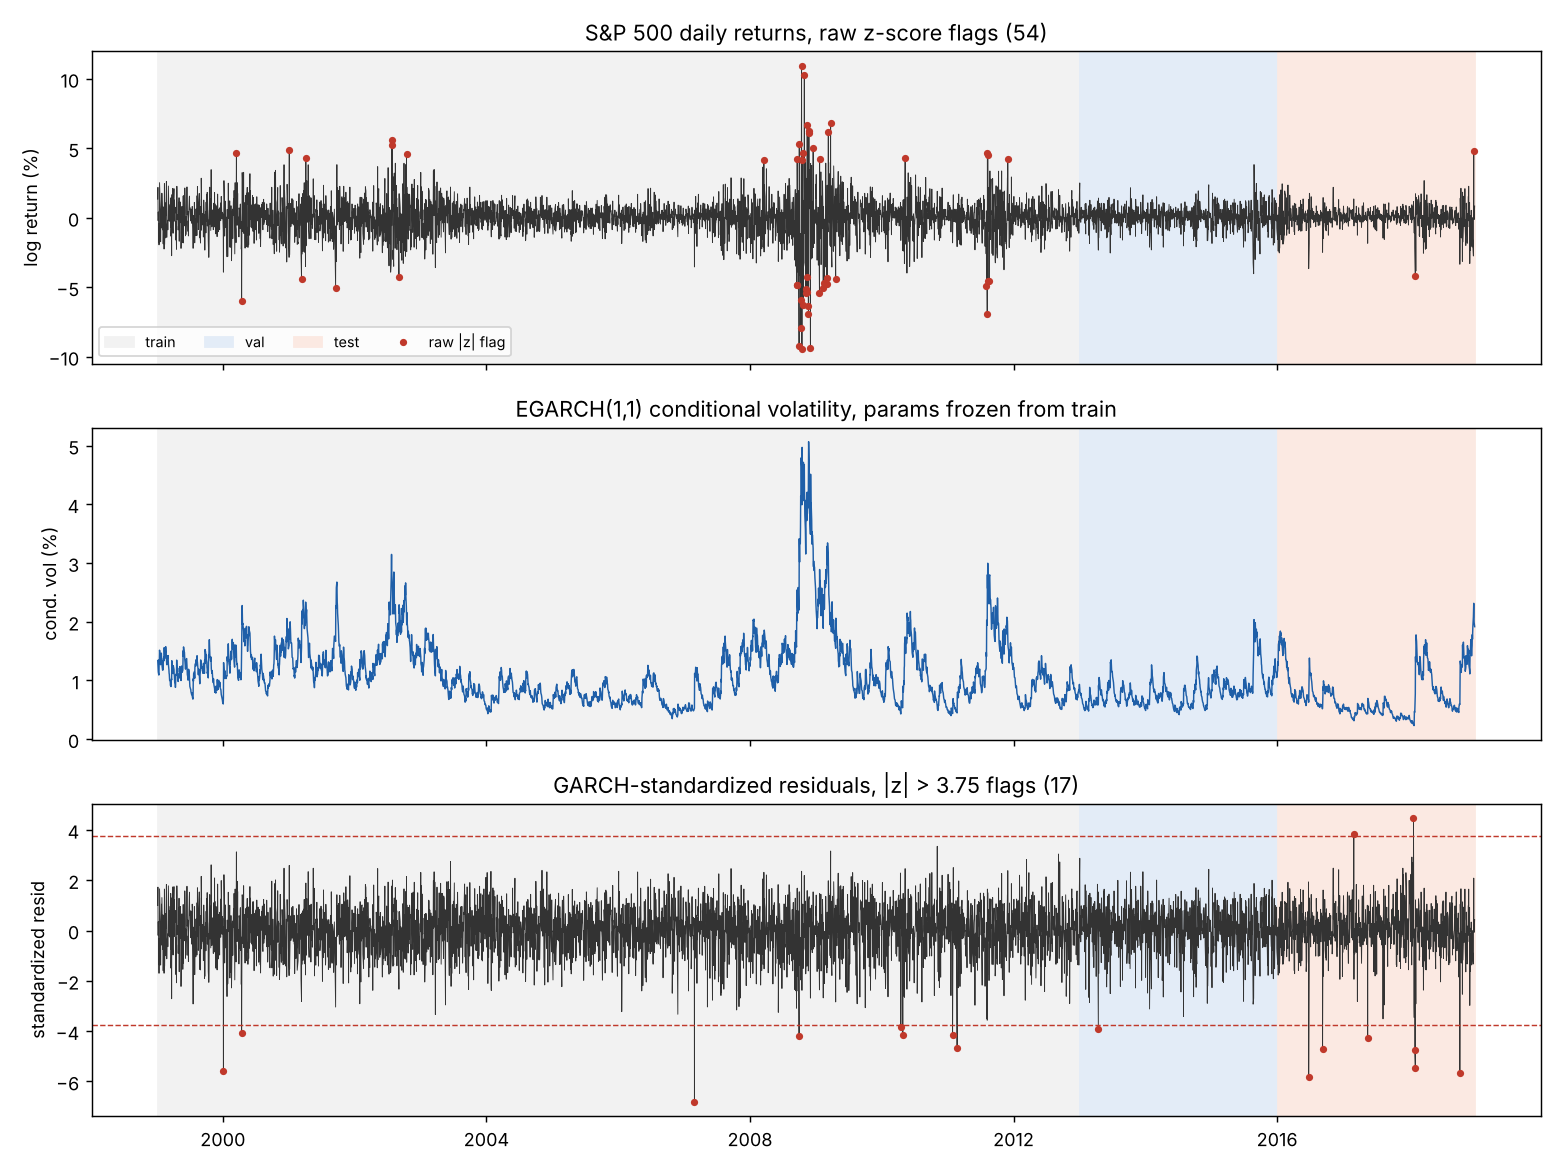
\includegraphics[width=\textwidth]{chapter4/figures/first_garch.png}
\caption{S\&P~500 daily returns with raw z-score flags (top), EGARCH conditional volatility
with parameters frozen from the training block (middle), and GARCH-standardized residuals
with flags beyond $|z|>3.75$ (bottom). Shading marks the training, validation and test
blocks.}
\label{fig:first-garch}
\end{figure}

The raw rule flagged 54 days, and 41 of them (76\%) fall in its three busiest years: 25 in
2008, 9 in 2009 and 7 in 2011. The rule mostly marks high-volatility periods rather than
individual days. The GARCH rule flagged 17 days, and its three busiest years hold 8 of them
(47\%). Its largest flags include 27 February 2007 (a global sell-off that began in
Shanghai), 29 September 2008 (the day the US House rejected the first bank rescue bill),
24 June 2016 (the day after the UK's Brexit referendum) and 5 February 2018 (a sharp rise in
US equity volatility). Of these four, the raw rule flags only the 2008 and 2018 days; the
2007 and 2016 moves were large for their own calm periods but not large compared with 2008.

One result shows a limit of the frozen-parameter setup. Eight of the 17 GARCH flags fall
in the 754 test days, where about 1.5 would be expected. In 2017 the filtered volatility
fell below anything seen in the training period (Figure~\ref{fig:first-garch}, middle
panel), so moderate moves in 2017 and early 2018 produced large standardized residuals. The
parameters, fixed at the end of 2012, do not adapt to this calmer regime. This is the
leakage-safe design behaving as intended, but it means the volatility model must be re-estimated on a rolling or expanding
window before statistical labels are fixed.

\subsection{Implications for the Main Experiments}
The preliminary run supports three decisions. The volatility model is chosen on validation
diagnostics, with GJR as the first candidate for the DSE. Statistical labels need periodic
re-estimation of the volatility model. Volatility standardization changes which days are
flagged, moving flags away from crisis periods towards days that were unusual for their own
period, which is the effect the autoencoder comparison will test. All three need to be
checked on DSE data.

\section{Expected Outcomes}
The main experiments have not been run. This section states what each hypothesis predicts
and what result would count against it, so that the results can be judged against
expectations fixed in advance.

\textbf{H1 (GARCH standardization).} The preliminary run shows that a threshold on raw
returns concentrates its flags in crisis years, while a threshold on standardized residuals
spreads them across the sample. If H1 holds, the raw-input autoencoder will show the same
pattern: more false alarms in the volatile regime and lower event-based F1 than the
standardized-input autoencoder. If the two autoencoders perform the same, or the raw model
does better on events labelled from market records, H1 is rejected for that label source.
A mixed outcome, in which standardization helps in some regimes and not others, is also
possible and will be reported as such.

\textbf{H2 (transfer).} If H2 holds, the zero-shot detector trained on global indices will
score above the statistical baselines on the DSE, and fine-tuning will narrow the gap to,
or exceed, the DSE-only detector. Standardized inputs are expected to transfer better than
raw ones, because removing each market's volatility level makes inputs from different
markets more comparable. If zero-shot transfer does not beat the baselines, the result will
show the limits of transfer into a frontier market with regulatory price distortions.

\textbf{H3 (point adjustment).} Given earlier findings on industrial
benchmarks~\cite{kim2022towards}, point-adjusted F1 is expected to exceed event-based F1 for
every detector, and the ranking of detectors may change between the two. A small gap would
also be informative: it would suggest that point adjustment matters less when most anomalies
last a single day.

\section{Main Results}
\todo{To be added after the experiments in Weeks 6 to 10: volatility model selection on DSE
data, baseline results, the raw versus standardized autoencoder comparison, transfer
results, the regime analysis and the evaluation gap.}

\section{Summary of the Chapter}
The preliminary run confirmed that the pipeline works end to end and led to three design
decisions: choose the volatility model on validation diagnostics, re-estimate it before
labels are fixed, and expect volatility standardization to move flags away from crisis
periods. The expected outcomes above set the criteria against which the main results will be
judged.


\chapter{Conclusion}
% Chapter 5: at the proposal stage this chapter holds the work plan, risks and fallbacks.
% At final submission it becomes the conclusion: findings, contributions, limitations and
% future work.

\section{Summary of the Proposal}
This thesis proposes to detect abnormal trading days on the Dhaka Stock Exchange with a
deep autoencoder whose inputs are returns standardized by GARCH-family conditional
volatility, and to train it on global market indices before transferring it to the DSE. The
work tests three hypotheses: that standardization improves detection and reduces false
alarms in volatile periods, that detectors transfer from global markets to the DSE, and that
point adjustment inflates reported performance on financial data. Phase~0 of the project is
complete: DSE data sources have been identified, 23 papers have been reviewed, the code
repository is set up, and a first volatility model run on S\&P~500 data has shaped the
design.

\section{Work Plan}
The work proceeds in five phases, each ending with a milestone that must be reached before
the next phase depends on it. Table~\ref{tab:plan} lists them in order.

\begin{table}[H]
\caption{Work plan.}
\label{tab:plan}
\begin{center}
\begin{tabular}{p{0.5cm} p{2.6cm} p{6.0cm} p{4.0cm}}
\hline
 & Phase & Work & Milestone \\
\hline
1 & Validation & DSE data sources identified (download not yet run); literature review
of 23 papers; first GARCH run; code repository and seed policy & Scope agreed with the
supervisor \\
2 & Proposal and setup & Research questions and hypotheses; global and DSE data collection;
DSE quality check & Proposal defended; DSE data pass the go/no-go criteria, or the
fallback market is chosen \\
3 & Data and labels & Cleaning (missing days, halts, floor prices, bonus shares, price
limits); GARCH, EGARCH and GJR fits with diagnostics; known-event, residual and injected
labels & Labelling rules fixed before any detector is trained \\
4 & Models and experiments & Baselines; raw versus standardized autoencoder; transfer
from global indices to the DSE; five-seed evaluation; regime analysis & All results
reported over five seeds \\
5 & Writing and submission & Thesis book; code release; data release if licensing allows;
IEEE paper draft & Thesis submitted \\
\hline
\end{tabular}
\end{center}
\end{table}

\section{Division of Work}
Each team member owns one strand of the work:
\begin{itemize}
    \item \textbf{\StudentTwoName:} data collection, cleaning and labels.
    \item \textbf{\StudentThreeName:} GARCH-family modelling and baselines.
    \item \textbf{\StudentOneName:} deep models and transfer experiments.
\end{itemize}
All three members write the thesis, with one member responsible for final integration.

\section{Risks and Fallbacks}\label{sec:risks}
\begin{itemize}
    \item \textbf{DSE data quality.} If the DSE pull fails the go/no-go criteria in
    Section~\ref{sec:dse-data}, the target market changes to India: the NIFTY~50 index and large-cap NSE
    stocks, which are available through \texttt{yfinance} with more than 15 years of
    adjusted daily data. India is an emerging market, not a frontier one, so the transfer
    question becomes weaker, and the thesis would say so.
    \item \textbf{Floor-price periods.} About two and a half of the 13 or so DSEX years fall
    under floor prices. If excluding them leaves too little normal data, results are
    reported both with and without them.
    \item \textbf{Scarce labels.} Real anomaly labels on the DSE are few. The three label
    sources reduce dependence on any one of them, and injected anomalies give a controlled
    test.
    \item \textbf{Negative results.} If standardization or transfer does not help, the
    thesis reports it, along with the regimes or markets in which it helps or hurts.
    \item \textbf{Data licensing.} The DSE website terms have not yet been reviewed. Until
    they are, the code and download scripts will be released but raw DSE prices will not.
    \item \textbf{Compute.} The models are small enough to train on a laptop or on free
    Colab or Kaggle GPUs.
\end{itemize}

\section{Expected Contributions}
\begin{enumerate}
    \item A controlled test of GARCH standardization as the input to a deep anomaly
    detector.
    \item The first deep, out-of-sample anomaly detection study on the DSE among the work
    reviewed, with documented handling of floor prices, bonus shares and price limits.
    \item Evidence on transferring anomaly detectors from global markets to a frontier
    market.
    \item A measurement of how much point adjustment inflates performance on financial data.
    \item Public code and, if licensing allows, labelled DSE series.
\end{enumerate}

\section{Concluding Remarks}
The preliminary run already shows the problem the thesis addresses: on raw returns, a
statistical rule flags crisis years, while on standardized returns it flags days that were
unusual for their own period. The next step is the DSE data pull, followed by the labelling
rules, which will be fixed before any detector is trained.


\renewcommand\bibname{References}
\bibliographystyle{IEEEtran}
\bibliography{backmatters/references}
\addcontentsline{toc}{chapter}{References}

%\chapter{Appendix}
\chapter*{}

\begin{center}
    \textbf{\LARGE APPENDIX A}
\end{center}

\vspace{1.5cm}  % You can adjust the space (e.g., 0.5cm, 2cm)

\noindent
Below are lists of contributions in form of publications and presentations: \\






%Appendix B
%insert here if you have several appendix
\chapter*{}

\begin{center}
    \textbf{\LARGE APPENDIX B}
\end{center}

\vspace{1.5cm}  % You can adjust the space (e.g., 0.5cm, 2cm)

\noindent Others Contribution: \\



\end{document}
